% Created by tikzDevice version 0.11 on 2018-07-20 11:37:01
% !TEX encoding = UTF-8 Unicode
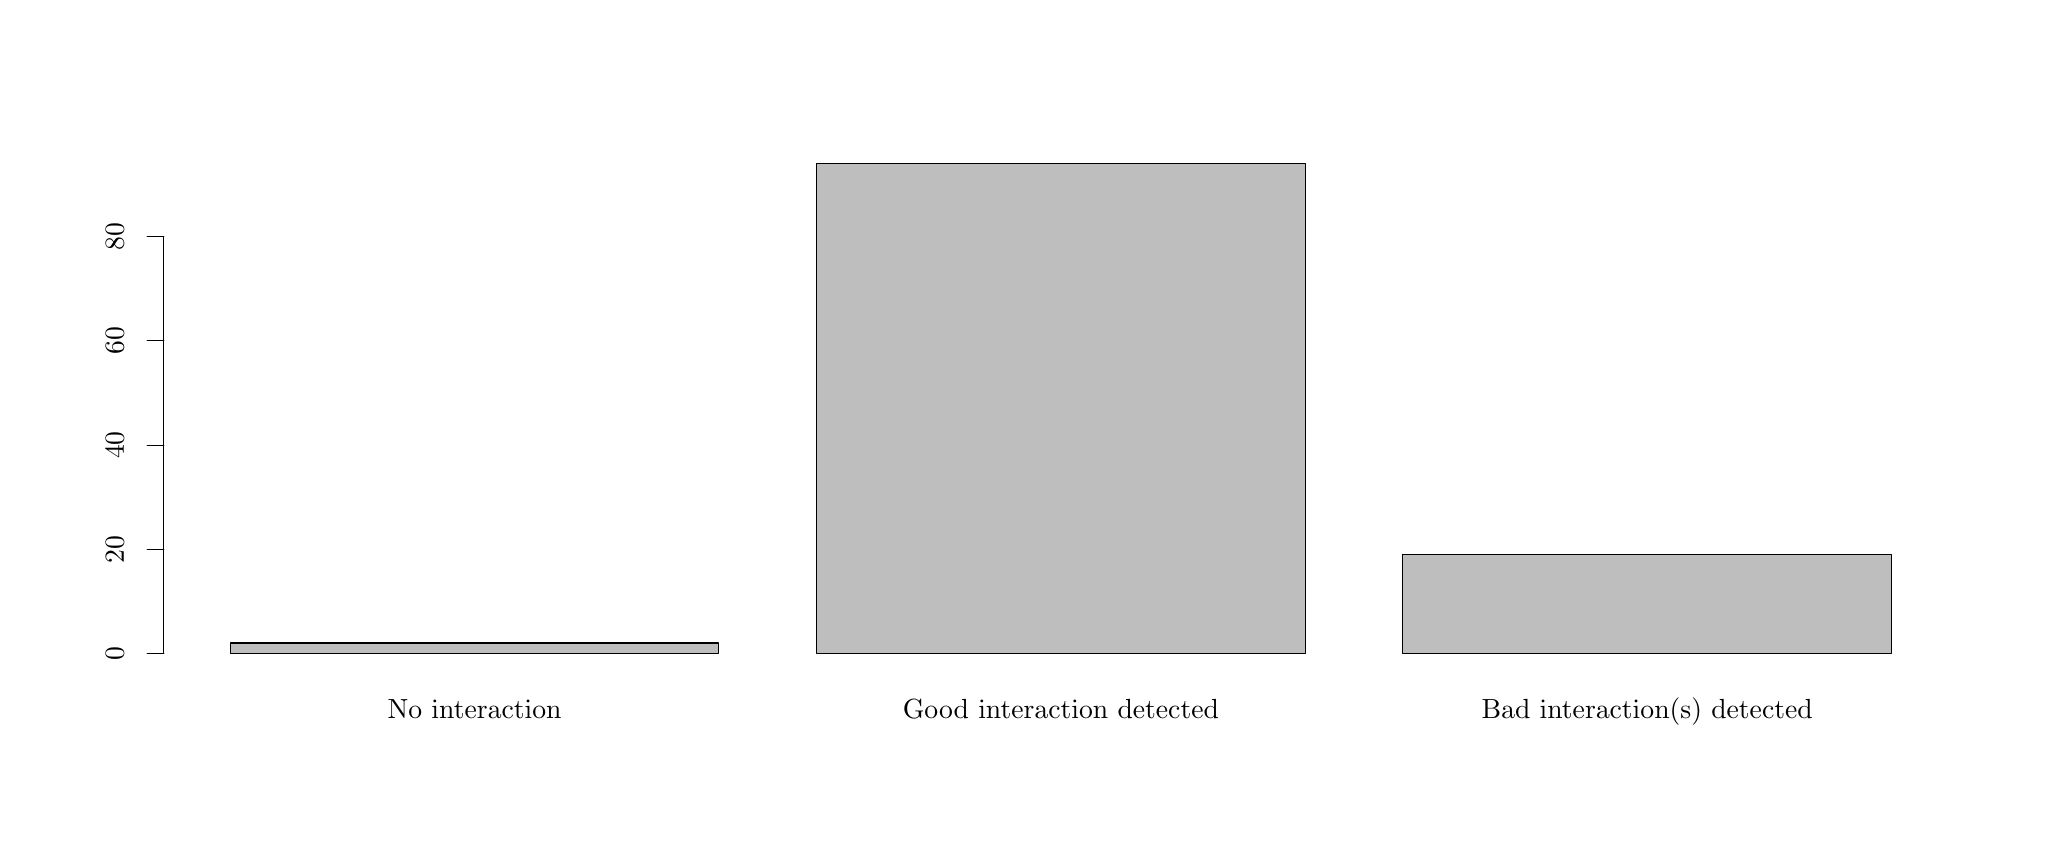
\begin{tikzpicture}[x=1pt,y=1pt]
\definecolor{fillColor}{RGB}{255,255,255}
\path[use as bounding box,fill=fillColor,fill opacity=0.00] (0,0) rectangle (722.70,289.08);
\begin{scope}
\path[clip] (  0.00,  0.00) rectangle (722.70,289.08);
\definecolor{drawColor}{RGB}{0,0,0}
\definecolor{fillColor}{RGB}{190,190,190}

\path[draw=drawColor,line width= 0.4pt,line join=round,line cap=round,fill=fillColor] ( 73.21, 62.97) rectangle (249.76, 66.73);

\path[draw=drawColor,line width= 0.4pt,line join=round,line cap=round,fill=fillColor] (285.07, 62.97) rectangle (461.63,239.88);

\path[draw=drawColor,line width= 0.4pt,line join=round,line cap=round,fill=fillColor] (496.94, 62.97) rectangle (673.49, 98.73);
\end{scope}
\begin{scope}
\path[clip] (  0.00,  0.00) rectangle (722.70,289.08);
\definecolor{drawColor}{RGB}{0,0,0}

\node[text=drawColor,anchor=base,inner sep=0pt, outer sep=0pt, scale=  1.00] at (161.49, 39.60) {No interaction};

\node[text=drawColor,anchor=base,inner sep=0pt, outer sep=0pt, scale=  1.00] at (373.35, 39.60) {Good interaction detected};

\node[text=drawColor,anchor=base,inner sep=0pt, outer sep=0pt, scale=  1.00] at (585.21, 39.60) {Bad interaction(s) detected};

\path[draw=drawColor,line width= 0.4pt,line join=round,line cap=round] ( 49.20, 62.97) -- ( 49.20,213.53);

\path[draw=drawColor,line width= 0.4pt,line join=round,line cap=round] ( 49.20, 62.97) -- ( 43.20, 62.97);

\path[draw=drawColor,line width= 0.4pt,line join=round,line cap=round] ( 49.20,100.61) -- ( 43.20,100.61);

\path[draw=drawColor,line width= 0.4pt,line join=round,line cap=round] ( 49.20,138.25) -- ( 43.20,138.25);

\path[draw=drawColor,line width= 0.4pt,line join=round,line cap=round] ( 49.20,175.89) -- ( 43.20,175.89);

\path[draw=drawColor,line width= 0.4pt,line join=round,line cap=round] ( 49.20,213.53) -- ( 43.20,213.53);

\node[text=drawColor,rotate= 90.00,anchor=base,inner sep=0pt, outer sep=0pt, scale=  1.00] at ( 34.80, 62.97) {0};

\node[text=drawColor,rotate= 90.00,anchor=base,inner sep=0pt, outer sep=0pt, scale=  1.00] at ( 34.80,100.61) {20};

\node[text=drawColor,rotate= 90.00,anchor=base,inner sep=0pt, outer sep=0pt, scale=  1.00] at ( 34.80,138.25) {40};

\node[text=drawColor,rotate= 90.00,anchor=base,inner sep=0pt, outer sep=0pt, scale=  1.00] at ( 34.80,175.89) {60};

\node[text=drawColor,rotate= 90.00,anchor=base,inner sep=0pt, outer sep=0pt, scale=  1.00] at ( 34.80,213.53) {80};
\end{scope}
\end{tikzpicture}
